\documentclass[10pt,a4paper]{article}
\usepackage[utf8]{inputenc}
\usepackage[OT4]{fontenc}
\usepackage{amsmath}
\usepackage{amsfonts}
\usepackage{amssymb}
\usepackage{titling}
\usepackage{anysize}
\usepackage{parskip}
\usepackage{graphicx}
\usepackage[polish]{babel}
\usepackage{float}
% some settings'

\setlength{\droptitle}{-2cm}
\preauthor{}
\DeclareRobustCommand{\authorthing}{
\begin{center}
\begin{tabular}{cc}
\large{Dominik Galewski} & \large{Jakub Woźniak} \\
106575 & 109686\\
dominik.galewski@student.put.edu.pl & jakub.l.wozniak@student.put.edu.pl
\end{tabular}\\
\vspace{8pt}
\large{Prowadzący: mgr inż. Mateusz Cicheński}\\
Wydział Informatyki Politechniki Poznańskiej
\end{center}}
\author{\authorthing}
\date{16 grudnia 2013}
\postauthor{}
\title{Trouble in Lecture Center\\\small{\MakeUppercase{Gra dungeon explorer}}\\\Large{Laboratorium Programowania Obiektowego}}
\marginsize{2cm}{2cm}{1cm}{1cm}

\setlength{\parindent}{0pt}
% document
\begin{document}
\maketitle


\section{Wprowadzenie}
\textbf{Trouble in Lecture Center} to gra typu \textit{dungeon explorer}, w której wcielamy się w postać studenta informatyki. Odwiedzając kolejne lokacje znajdujące się w mrocznych podziemiach jego uczelni, próbujemy zmierzyć się ze wszystkimi przeciwnościami: analizą matematyczną, programowaniem deklaratywnym, systemami operacyjnymi czy metodami probabilistycznymi. Nasze decyzje wpływają na los studenta i wynik starć z przeciwnikami.


\section{Struktura projektu}
\subsection{Instrukcja kompilacji}
Projekt został napisany w języku C++ (standard C++11) przy użyciu biblioteki \textit{SFML} (http://sfml-dev.org) w wersji 2.0. Do kompilacji wymagany jest kompilator g++ w wersji 4.8. Dostarczony plik \textit{Makefile} pozwala na skompilowanie projektu przy pomocy polecenia \textit{make}. Plik wynikowy znajduje się w katalogu \textit{bin}. Program należy uruchomić bedąc w katalogu \textit{bin/}, w przeciwnym razie nie zostaną załadowane pliki z grafiką, itp.

\subsection{Podział klas}
Rysunek \ref{uml-game} przedstawia podział klas związanych z rozgrywką. Główną klasę stanowi \textit{Entity}, która reprezentuje wszystkie elementy w grze, które mogą być narysowane na mapie. Klasa NPC przedstawia postacie sterowane przez komputer, obecnie istnieje tylko jedna klasa pochodna - \textit{HostileNPC}, które reprezentuje postacie wrogie użytkownikowi. Klasa \textit{Player} odpowiada za reprezentowanie postaci gracza w grze, dzieli się na 3 klasy pochodne, które są profesjami postaci. \textit{DMG} --- wyświetla zadane obrażenia na mapie.

Rysynek \ref{uml-game2} przedstawia zależność klas związanych z logiką gry, głównie reprezentuje klasę \textit{IState} i jej klasy pochodne --- odpowiednie stany w których gra może się znajdować (splash, tworzenie postaci, intro, menu, gra właściwa, zakończenie). Dodatkowo, klasa \textit{GameState} zawiera pole typu \textit{Level} będące obiektem reprezentującym aktualnie rozgrywany poziom.

Rysunek \ref{uml-game3} przedstawia pozostałe klasy: \textit{Engine} --- zawierająca logikę uruchomienia i utrzymania pętli zdarzeń wraz z przekazywaniem kontroli do stanów, \textit{Log} --- prosty interfejs do zapisywania logu, \textit{StateManager} --- maszyna stanów, odpowiadająca za przechowywanie i zarządzanie obiektami stanów gry, \textit{SoundManager} --- klasa zarządzająca dźwiękiem w grze.

\begin{figure}
    \centering
    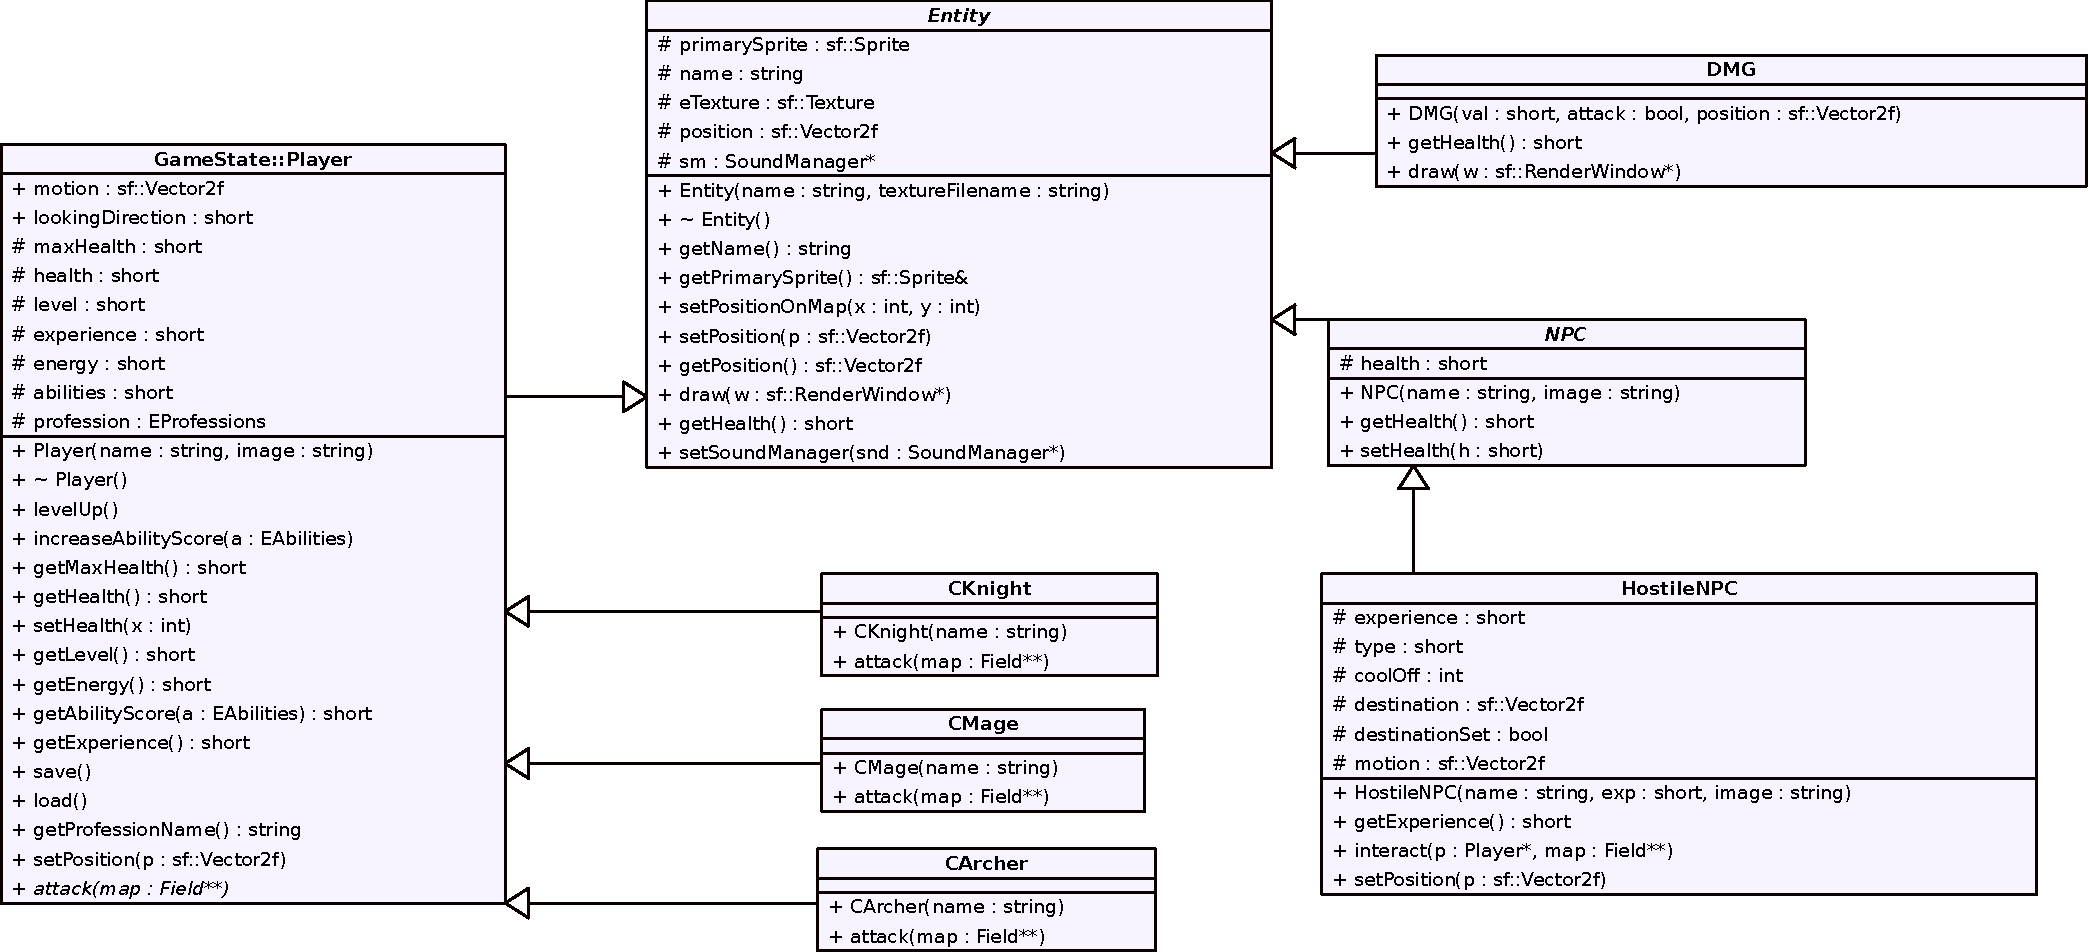
\includegraphics[width=\textwidth]{uml/class1.pdf}
    \caption{diagram podziału klas związanych z rozgrywką}
    \label{uml-game}
\end{figure}

\begin{figure}
    \centering
    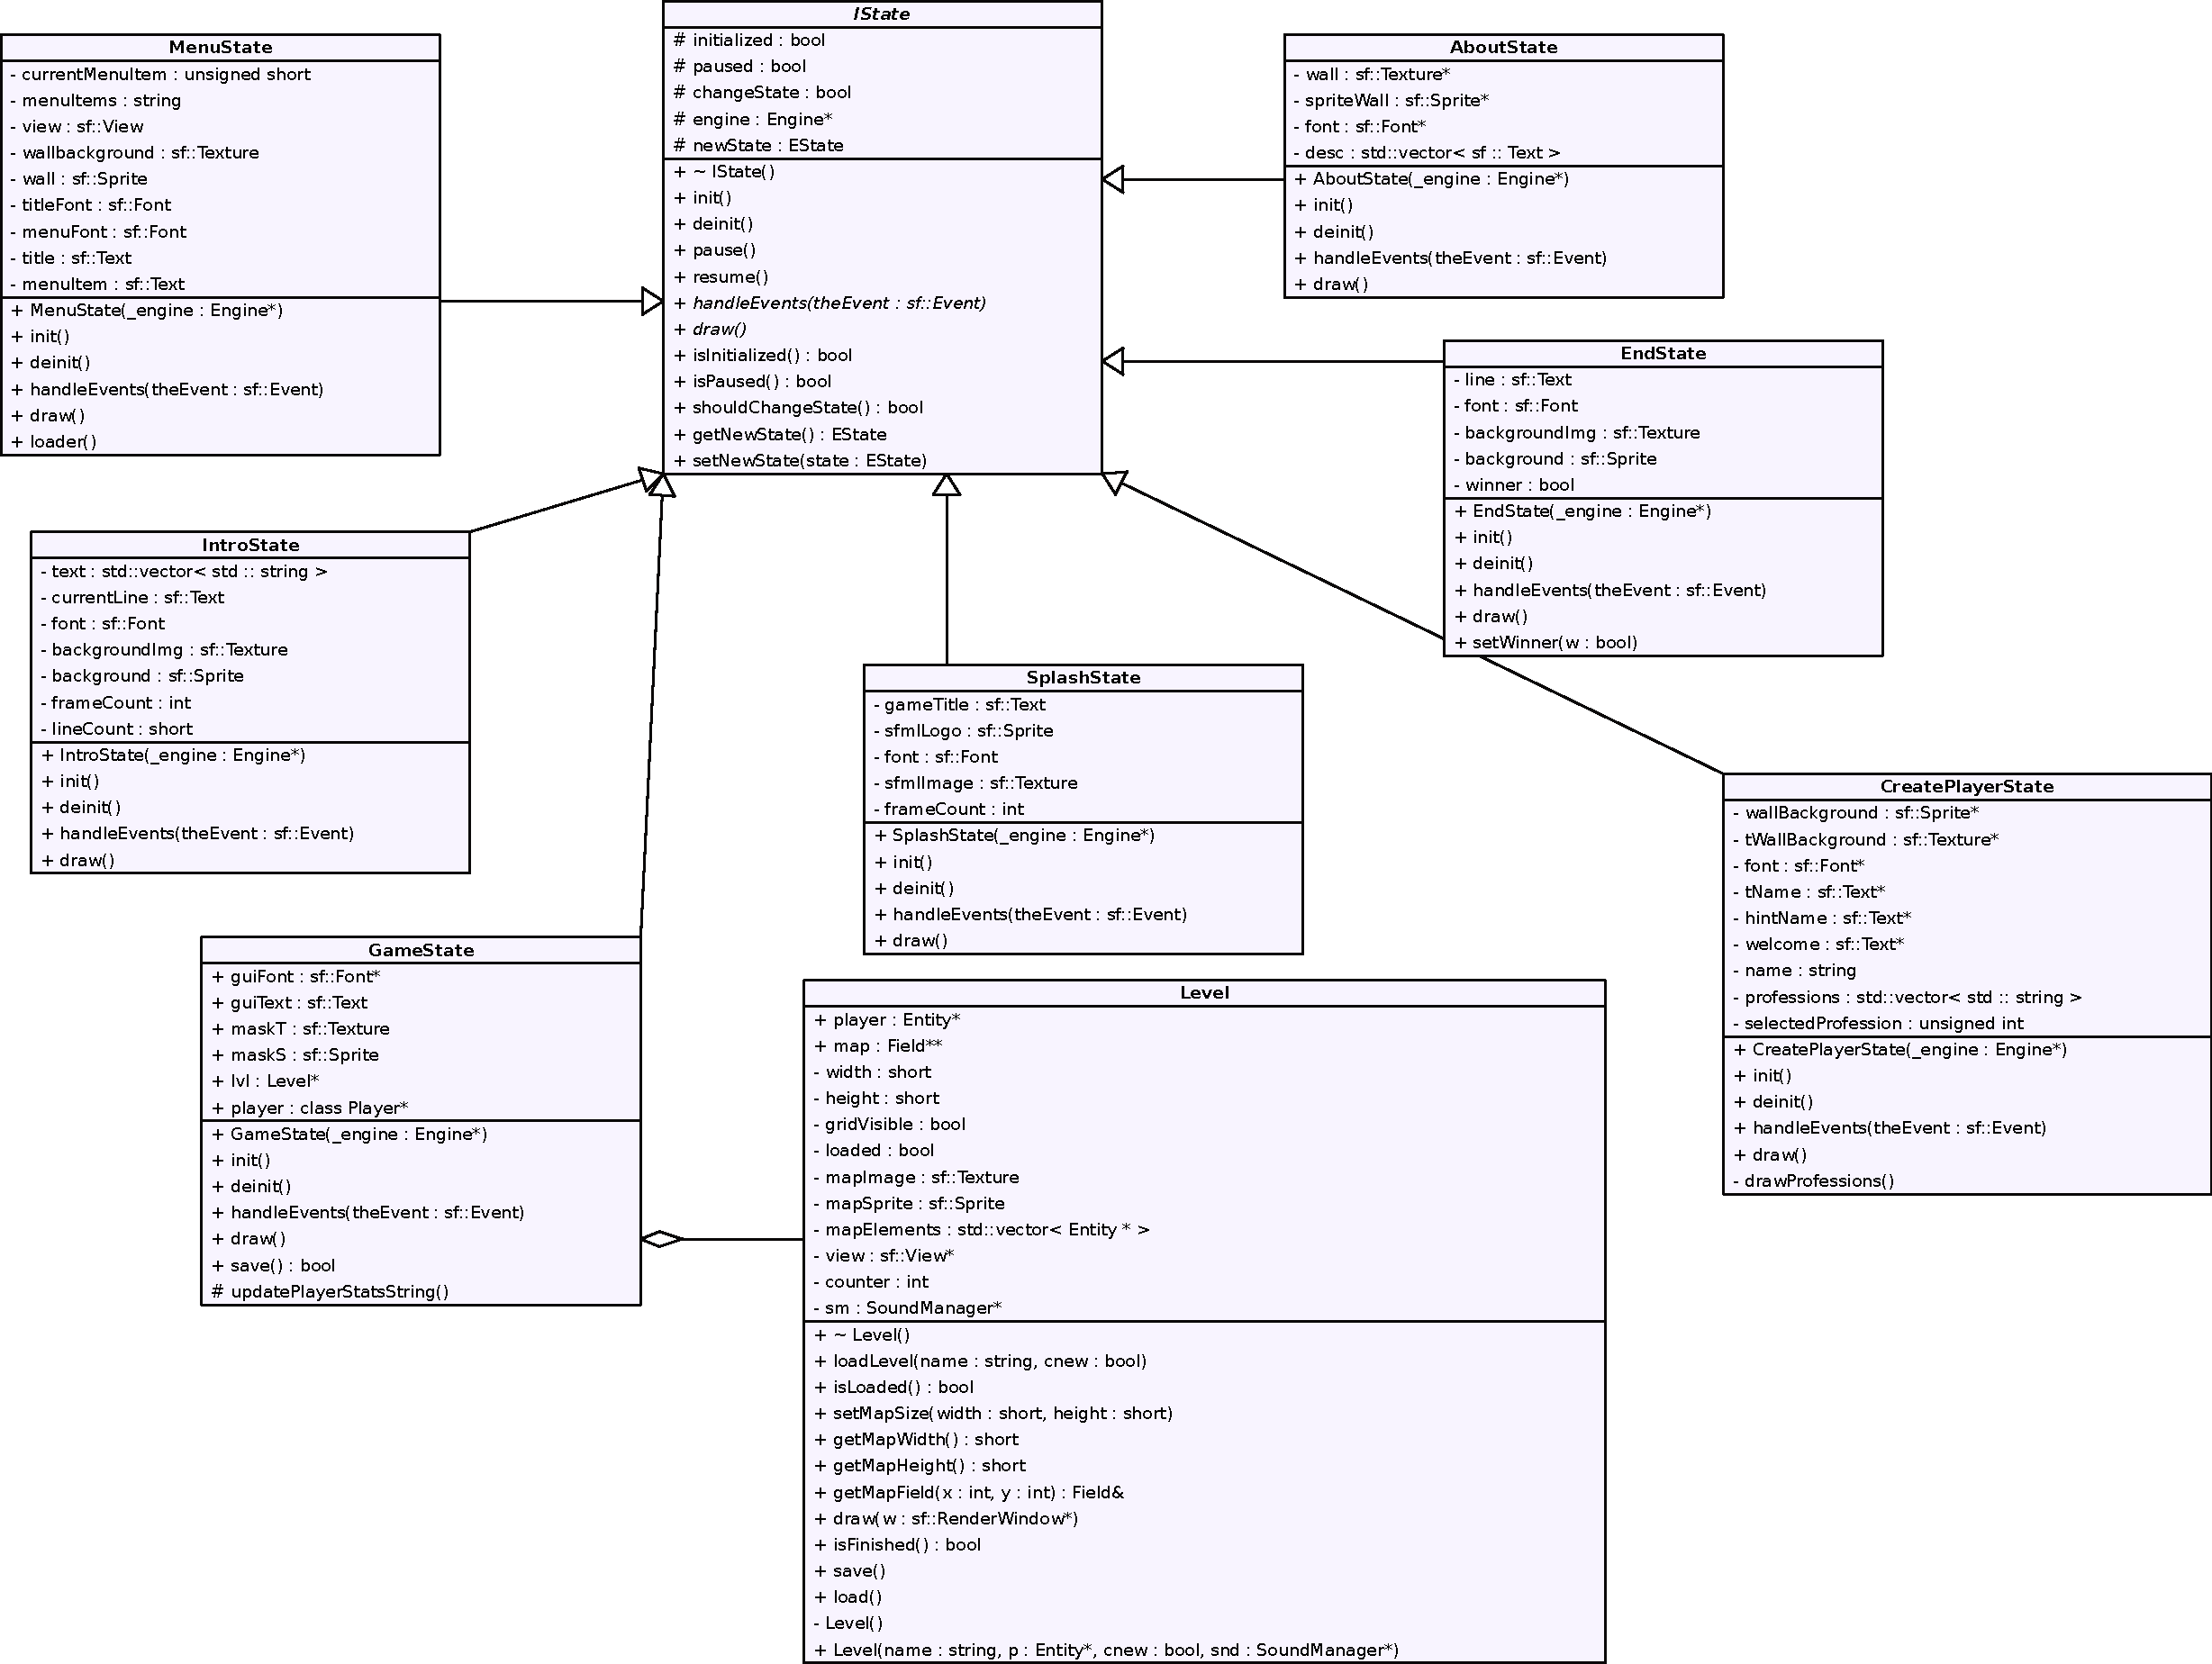
\includegraphics[width=\textwidth]{uml/class2.pdf}
    \caption{diagram podziału klas związanych z logiką}
    \label{uml-game2}
\end{figure}

\begin{figure}
    \centering
    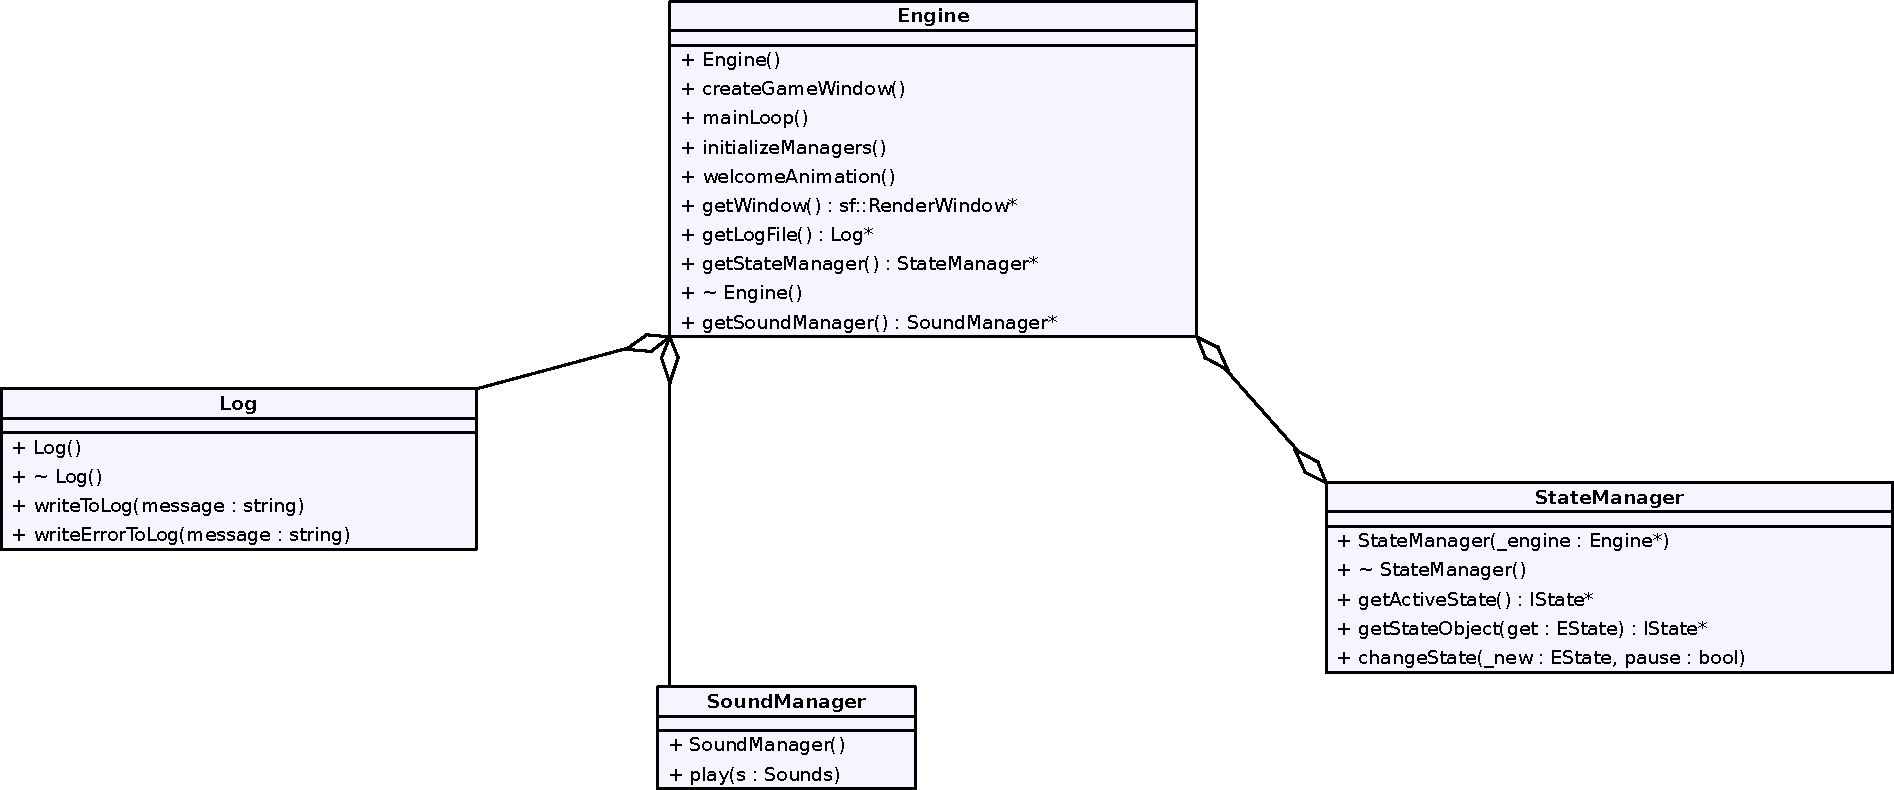
\includegraphics[width=\textwidth]{uml/class3.pdf}
    \caption{diagram podziału pozostałych klas}
    \label{uml-game3}
\end{figure}

\subsection{Klawiszologia}
Postać porusza się przy pomocy klawiszy \textit{WSAD}, atakuje przy pomocy \textit{Spacji}. Natychmiastowy powrót do menu gry następuje poprzez wciśnięcie klawisza \textit{Esc}, a zapis gry przy pomocy \textit{F5}.

\section{Spis wymagań}
\subsection{Graficzny interfejs użytkownika}
Interfejs użytkownika został zrealizowany przy pomocy biblioteki \textit{SFML}. Wykorzystane elementy graficzne i dźwiękowe zostały wykonane przez nas lub są na wolnej licencji. Mapa zrealizowana jest w widoku ,,z lotu ptaka''.

\subsection{Wpływanie na rozgrywkę}
Użytkownik dokonuje wyboru profesji, taktyki i sposobu walki z przeciwnikiem tak, aby pokonać wszystkich wrogów. Musi unikać ciosów, atakować w odpowiednich momentach i uważać na możliwość zablokowania przez wrogie jednostki.

\subsection{Zapis stanu gry}
Użytkownik w każdym momencie gry ma możliwość zapisu aktualnego stanu celem późniejszego odtworzenia.

\end{document}
